\documentclass[11pt]{report}

%to allow more levels of sections and paragraphs:
\setcounter{secnumdepth}{4}

%Packages
\usepackage[utf8]{inputenc}
\usepackage[breaklinks=true,hidelinks]{hyperref}
\usepackage{graphicx}
\usepackage[spanish, english]{babel}
\usepackage{url}
\usepackage{multirow}
\usepackage{verbatim} %comentarios
\usepackage{amsmath}
\usepackage{amssymb}
\usepackage{textcomp,gensymb}
\usepackage{colortbl}
\usepackage{graphicx} % Para escalar la tabla
\usepackage[table,xcdraw]{xcolor}
\usepackage{multirow}
\usepackage{diagbox}
\usepackage{dashrule}
\usepackage{pdflscape}
\usepackage{fancyhdr} % Para personalizar encabezados y pies
\usepackage[T1]{fontenc}

\usepackage{multicol} 

\usepackage{subfig}

\usepackage{rotating}

\usepackage{pifont}

\usepackage{relsize}
\usepackage{xcolor,colortbl}
\usepackage{wrapfig}
\usepackage{bbm}
\usepackage[labelfont=bf]{caption}
\usepackage{tabularx}

\DeclareMathOperator{\arctantwo}{arctan2}

\graphicspath{ {img/} }

\usepackage[document]{ragged2e}
\usepackage{float}
\usepackage{listings}
\usepackage[left=3cm, right=3cm, top = 2.5cm, bottom = 2.5cm, includehead, includefoot]{geometry}

\usepackage{titlesec}

\usepackage{appendix}
\usepackage{minted}
\usepackage{afterpage}
\usepackage{xparse}

\usepackage{algorithm}
\usepackage[noend]{algpseudocode}

\usepackage{eurosym}

\setlength{\headheight}{32.09pt}

%Config
\setlength{\parskip}{1em}
\setlength{\parindent}{0em}

\titleformat*{\section}{\color{black}\bfseries\Large}
\titleformat{\chapter}[display]
{\normalfont\bfseries}{}{0pt}{\Huge}

\makeatletter
    \renewcommand*\@makechapterhead[1]{
        {\Huge\bfseries #1\par \nobreak\vskip 60\p@}
    }
\makeatother
 
\usepackage{pdflscape}
\usepackage{lscape}
\usepackage{afterpage}
% =====Añadido por mí=====
\usepackage{todonotes}
\setuptodonotes{inline}
\usepackage{minted}
\usepackage{dirtree}
\newcommand{\review}[2][]{%
  \todo[color=red!50,#1]{#2}%
}
\newcommand{\notes}[2][]{%
  \todo[color=blue!25,#1]{#2}%
}
% ==========
\begin{document}

\selectlanguage{spanish}

\renewcommand{\contentsname}{Índice}
\renewcommand{\partname}{Parte} 
\renewcommand{\chaptername}{Chapter} 

\renewcommand{\appendixname}{Apéndice} 
\renewcommand{\figurename}{Figura}
\renewcommand{\tablename}{Tabla} 
\renewcommand{\listfigurename}{Índice de figuras} 
\renewcommand{\glossaryname}{Glosario}


\begin{titlepage}

\newgeometry{top=2.5cm, left=2cm, right=2cm}

\definecolor{customOrange}{HTML}{ff6500}

\pagecolor{customOrange}\afterpage{\nopagecolor}


\begin{center}

 { \huge \textbf{UNIVERSIDAD POLITÉCNICA DE MADRID} \par} 

 {\vspace{0.5cm}}
 
 {\scshape  \Large \textbf{ESCUELA TÉCNICA SUPERIOR \\ DE INGENIEROS DE TELECOMUNICACIÓN} \par} 



    {\vspace{1.5cm}}
    
    
\begin{figure}[H]
    \centering
    
\includegraphics[scale=0.3]{img/logoBN3.png}
    \label{logoNegro}
\end{figure}{}
 
 
   {\vspace{1cm}}


    { \vspace{1.5cm} \Large \textbf{GRADO EN INGENIERÍA Y SISTEMAS DE DATOS}}

    { \vspace{0.5cm} \Large \textbf{TRABAJO FIN DE GRADO}}

    {\vspace{1cm}}
 
   {\scshape  \Large \textbf{Aplicación de técnicas de Machine Learning para la identificación y optimización de 
patrones en 'Swing Chart' en mercados financieros} \par} 
   
   
   
   
   
   \vspace{1.5cm}
   {\itshape \Large \textbf{Lijun Zhou} \par}
   
   
   
  \vspace{1cm}
  \Large \textbf{2026} \par


  
   
\end{center}


\restoregeometry
\end{titlepage}

\pagenumbering{gobble} %Quitar numeracion

\null\clearpage % WhitePage

\pagenumbering{gobble}

\LARGE \textbf{Grado en Ingeniería y Sistemas de Datos}

\vspace{0.5cm}

\LARGE \textbf{TRABAJO DE FIN DE GRADO}

\vspace{0.5cm}

\large \textbf{Título}: Aplicación de técnicas de Machine Learning para la identificación y optimización de 
patrones en 'Swing Chart' en mercados financieros

\large \textbf{Autor}: D. Lijun Zhou

\large \textbf{Supervisión técnica}: 

\large \textbf{Supervisión académica}: Dr. Eduardo López Gonzalo 

\large \textbf{Departamento}: Departamento de Señales, Sistemas y Radiocomunicaciones.

\vspace{0.5cm}

\LARGE \textbf{MIEMBROS DEL TRIBUNAL}

\vspace{0.5cm}
\large \textbf{Presidente}: \hdashrule[0.5ex]{5cm}{1pt}{2pt}

\large \textbf{Vocal}: \hdashrule[0.5ex]{6cm}{1pt}{2pt}

\large \textbf{Secretario}: \hdashrule[0.5ex]{5.1cm}{1pt}{2pt}

\large \textbf{Suplente}: \hdashrule[0.5ex]{5.4cm}{1pt}{2pt}

\vspace{2cm}

\normalsize \textbf{Los miembros del tribunal arriba nombrados acuerdan otorgar la calificación de:}

\vspace{1cm}

\hdashrule[0.5ex]{6cm}{1pt}{2pt}

\vspace{1cm}

\large \textbf{Fecha de lectura}: \hdashrule[0.5ex]{5cm}{1pt}{2pt}

\normalsize

\clearpage




\null\clearpage % WhitePage

\input{intro/cover.tex}

\null\clearpage % WhitePage


% Page header and footer
\pagestyle{fancy}

\fancyhf{}
\lhead{
\begin{picture}(0,0)
    
\includegraphics[scale=0.04]{img/logoescuela.jpg}
\end{picture}{}
}
\rhead{\thepage}
% End

\justifying


\setlength{\parindent}{0em}
\pagenumbering{gobble}

\section*{Resumen}

El trabajo presenta el diseño, implementación y evaluación de un sistema de trading algorítmico basado en técnicas de Machine Learning para la
identificación y optimización de movimientos LONG/SHORT aplicados a futuros financieros. El objetivo principal es operar de forma autónoma una
cartera diversificada (valor objetivo de 1 millón USD) sobre 13 contratos de futuros (divisas, índices, materias primas y bonos), maximizando
beneficio y controlando riesgo. La arquitectura propuesta es híbrida: combina modelos supervisados (LSTM y GRU) para generar señales direccionales y
una capa de regresión para estimar retornos.

El flujo de datos sigue un pipeline ETL organizado en capas Bronce-Plata-Oro: ingestión de datos OHLCV minuto a minuto, limpieza y estandarización
temporal a UTC, resampleo a velas de 4 horas y cálculo de un amplio conjunto de features (momentum, volatilidad, volumen, estructurales y derivados de
swing charts). Se aplica selección de características (correlación, LASSO) para reducir dimensionalidad y evitar data leakage. La etiqueta objetivo se
construye con el método de triple barrera (Stop Loss, Take Profit, vencimiento temporal) y se complementa con la regresión del retorno logarítmico.

Los modelos se entrenan con PyTorch usando una estrategia walk-forward (moving window) para respetar la estructura temporal y evitar fugas. La
solución consta de tres niveles: L1 (detección de movimiento significativo), L2 (dirección BUY/SELL) y L3 (regresión de retorno); la decisión final se
obtiene por soft-voting ponderado por el retorno estimado. Se emplea RobustScaler y técnicas de regularización (dropout) para garantizar la robustez
frente a outliers y cambios de régimen.

El backtest se realiza sobre datos de 4 horas y contempla fases de selección de predicciones y simulación operativa con distintas modalidades
(long/short, scale-in, sizing dinámico). Las métricas evaluadas incluyen Sharpe, Max Drawdown, Calmar y CAGR; además se usan simulaciones Monte Carlo
para analizar robustez y sensibilidad. Para despliegue se dockeriza el sistema e integra monitorización con Prometheus/Loki, visualización en Grafana
y alertas vía Slack. El trabajo incluye análisis ético y económico, resultados de entrenamiento y backtests, y propone líneas futuras como aprendizaje
no supervisado, orquestación MLOps y optimización con Pyomo.

\section*{Palabras clave}

Trading algorítmico, Swing Charts, Machine Learning, LSTM, GRU, Triple barrera, Walk-forward, Feature engineering, Backtesting, Monte Carlo, RobustScaler, Dockerización, Grafana, Gestión de riesgo, Selección de características (LASSO)
\clearpage

\setlength{\parindent}{0em}
\pagenumbering{gobble}
%\chapter*{}\label{sum}\thispagestyle{fancy}

\section*{Summary}

XXXXXXXX

\section*{Keywords}

XXXXXXXX

\clearpage

%\setlength{\parindent}{0em}
\pagenumbering{gobble}
\thispagestyle{fancy}

\noindent% prevent the box to be shifted a bit to the right
\makebox[\textwidth][r]{% create a box, with it's content aligned to the right
  \begin{minipage}{.5\textwidth}% create a content half width
    \section*{Agradecimientos}
    \justifying
    \textit{Si quieres poner dedicatoria, descomentar en main.tex.}

  \end{minipage}
}
%\clearpage\null\newpage

\clearpage
\clearpage

\pagenumbering{gobble}

\fancypagestyle{plain}{
  \thispagestyle{fancy}
  \renewcommand{\contentsname}{Índice}
}

\tableofcontents

\clearpage %%% Quita esto si no quieres las figuras
\renewcommand{\listfigurename}{Listado de figuras}
\listoffigures

\clearpage %%% Quita esto si no quieres las tablas
\renewcommand{\listtablename}{Listado de tablas}
\listoftables

\clearpage



\clearpage\null\newpage
\setlength{\parindent}{0em}
\pagenumbering{gobble}


\section*{Glosario}

\textbf{OHLCV} - Precios Open High Low y Close y Volumen

\textbf{XXXX}	       -  XXXXXXXX

\clearpage\null\newpage

\pagenumbering{arabic}

%%%%% CUERPO DEL DOCUMENTO %%%%%%%

\setlength{\parindent}{0em}

\chapter{Introducción y objetivos}\label{cap1}\thispagestyle{fancy}

\vspace{-1.3cm}

\section{XXXXXXXXXX}

\section{XXXXXXXXXX}



\setlength{\parindent}{0em}

\chapter{Estado del arte}\label{cap2}\thispagestyle{fancy}

\vspace{-1.3cm}

\section{XXXXXXXXXX}

\notes{Quizás explicar lo que son LSTM y GRU aunqe sean bastante antiguos}

Los dos modelos de aprendizaje automático profundo que se van a implementar en este trabajo son dos Redes Neuronales Recurrentes \cite{elman1990rnn}, un
tipo de red presentada en 1990, apartir de ahí se han creado diferentes redes mejoradas, de las dos mencionadas primero se publicó el paper de LSTM
(Long-Short Term Memory) \cite{hochreiter1997lstm} en 1997 y después, GRU (Gated Recurrent Unit) en 2014 \cite{cho2014gru}


\setlength{\parindent}{0em}

\chapter{Desarrollo}\label{cap3}\thispagestyle{fancy}

\vspace{-1.3cm}

\section{Desarrollo del autómata}

El desarrollo del sistema se divide en diferentes fases dentro de la ETL, destacando la carga de datos históricos, su limpieza y filtrado,
su transformación en las diferentes características para alimentar a los modelos de aprendizaje automático.

% Además, están las partes de 

% Se quiere usar una arquitectura de medallón, para representar la utilidad de los datos, en primer lugar están los datos en crudo que se cargan

El objetivo es poder generalizar el código, que no importe de qué activos sean los datos el flujo de datos puede reutilizarse.

Para lograr este objetivo he decidido implementar la lógica del código dentro de un paquete instalable de python usando
\mintinline{bash}{pip install -e} y he decidido usar la siguiente estructura organizativa.

\dirtree{%
    .1 /.
    .2 paths.py.
    .2 get\_info.
    .2 data.
        .3 loader.py.
        .3 cleaner.py.
        .3 resampler.py.
        .3 to\_parquet.py.
    .2 features.
    .2 supervised.
    .2 unsupervised.
    .2 portfolio.
    .2 risk.
    .2 execution.
    .2 logging.
    .2 retrain.
}

Hay funciones que están en algunos de los directorios que pueden servir para varias entapas del proceso, principalmente aquellas encargadas de
obtener los datos desde los archivos.

A continuación paso a explicar cada una de las fases del flujo de los datos y las funciones utilizadas en ellas.

\subsection{Carga y limpieza}

Se me han facilitado los datos históricos OHLCV de distintos futuros con los que voy a operar.

En un primer análisis me doy cuenta de que los datos temporales no están regularizados al formato UTC, por lo que es el primer cambio que realizo.
Usando de referencia las horas de apertura y cierre de cada futuro, agrupo el volumen por horas para cada activo puedo detectar las horas con poca
o nula actividad, con ello puedo inferir la zona horaría usada.

\todo{Explicar mejor cómo funciona la función de inferencia}

Después, decido filtrar los datos que claramente no deberían de estar, estos son los que aparecen en los fines de semana. Los pedidos realoizados en
las horas de descanso las mantengo por que pueden haber sido retrasos en la ejecución por lo que son operaciones reales no realizadas en el momento
indicado.

Una vez estandarizado el tiempo aprovecho la función de inferencia y añado una priemra columna derivada que indica el día de \textit{trading} aunque
al ser una fecha no se usará directamente para el entrenamiento si me ayudará para calcular valores acumulados diarios.

Por otra parte como mi intención es obtener métricas de comparación entre activos decido recortar el número de filas disponibles en los diferentes
archivos para tener un conjunto homogéneo. Además para mejorar el rendimiento y disminuir el tamaño de los archivos convierto los datos que estaban
en formato csv a parquet.

\subsection{Cálculo de características}

Una vez con los datos OHLCV limpios, llega el momento de aplicar diferentes funciones de diversas librerías para obtener características derivadas
que servirán para alimentar a los modelos.

Hay características de diferentes tipos, momento, estructural, temporal, de tendencia, de volatilidad, de volumen y características derivadas de
otras. Al ser una estratégia multidía también he hecho uso de los swing charts y de características derivadas de ellas, además de otras
características obtenidas de comparar diferentes activos

Para obtener estas características primero agrupo los datos que venían minuto a minuto a agrupaciones de 4 horas, de esto modo se evita tener el
ruido de señales tan cortas y es un buen número para una estratégia interdía donde una posición puede estar abierta varios días

\subsection{Selección de características}

Una vez calculadas todas las características es necesario reducir ese número porque es posible que muchas de ellas estén interrelacionadas

Para ello se aplican varias técnicas, empezando por la más básica, un filtro de alta correlación, además de eliminar las características que puedan
predecir el futuro, las no cíclicas o no estacionarias pueden confundir a los modelos indicando que en valor que quizás representaba el día de la
semana sea considerado como más importante a mayor número

También filtro usando el algorítmo de LASSO usando un modelo de aprendizaje automático clásico de sklearn que permité mayor explicabilidad

\subsection{Aprendizaje supervisado}

El uso de modelos de aprendizaje supervisado se centra en modelos de clasificación binaria, en este caso en dos etapas, y dentro de cada etapa se
utilizan dos modelos de aprendizaje profundo usando PyTorch, LSTM y GRU. Cada uno de los modelos utilizados tiene una función, LSTM ..., por su parte GRU.
Para ambas fases se realiza una votación equitativa, si la media supera el umbral indicado para cada fase se pasa a la siguiente
\notes{Probar a ver otros métodos de votación además de usar la media}

Existe una tercera etapa, en este caso de regresión que sigue la misma lógica, usando los dos modelos

\subsection{Aprendizaje no supervisado}

Pasando ahora a los modelos, primero voy a explicar las dos situaciones donde voy a implementar modelos de aprendizaje no supervisado

En primer lugar para agrupar los diferentes activos en diferentes grupos. En vez de realizar agrupaciones arbitrarias por ejemplo todas las monedas
juntas dejo que el sistema decida cuales son los activos más parecidos

\todo{Decidir el algoritmo a usar para UL}
% \review{Prueba cuadro \textbackslash review}

\section{Despliegue usando contenedores de Docker}

Una vez que se ha desarrollado el autómata y se ha comprobado que su funcionamiento es correcto, he decidido añadir el proyecto a un contenedor de
docker para facilitar el despligue en otros equipos

\subsection{Configuración del contenedor principal}

Por cómo he desarrollado el sistema y por velocidad todo va a estar incluido en un único contenedor.

No requiere demasidos cambios ya que voy a copiar los códigos desarrollados dentro del contenedor

\subsection{Bases de datos}

Al tener el proyecto dentro de un contenedor veo lógico tener una base de datos con diferentes tablas para guardar diferentes métricas

\subsection{Alertas y avisos}

Por último una vez que todo funciona en contenedores he decidido añadir un sistema de visualización de toda la información que se recopila en
directo y en diferido

Uso Prometheus, Grafana y Alertmanager este último conectado a otro servicio que se conecta a la API de whatsapp

\subsection{Orquestación y MLOps}

\notes{Tanto Airflow como MLflow, ver si hay tiempo para implementarlos}

Una vez desplegado un sistema robusto que cuenta con un autómata funcional y con alertas tanto de seguridad como para mostrar información, decido
implementar el uso de Airflow como orquestrador.

En general el uso de Airflow está muy ligado al uso de MLflow ya que será el uso prinicpal de esta herramienta por mi parte.

En MLflow 

% \subsection{MLOps}

% Uso de MLflow

\setlength{\parindent}{0em}

\chapter{Resultados}\label{cap4}\thispagestyle{fancy}

\vspace{-1.3cm}

\section{Resultados}

Como se han mencionado en cápitulos anteriores el resultado de las pruebas ha sido positivo

En la gráfica siguiente se muestra cómo va evolucionando el capital de la cuenta simulada, se puede observar todas las predicciones que realizan los
modelos y el sharpe ratio final.

\begin{figure}[h]
    \centering
    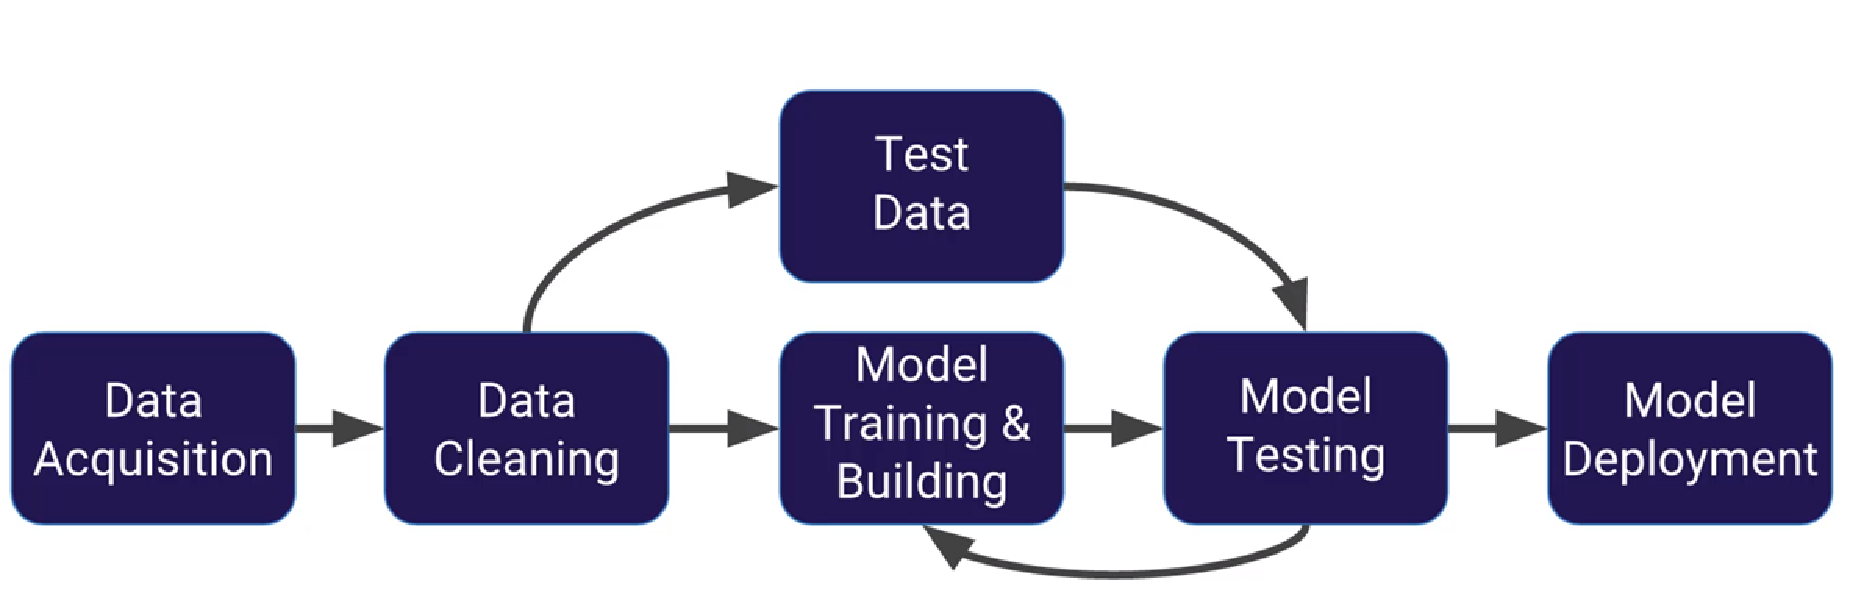
\includegraphics[scale=0.45]{./img/ml_process.pdf}
    \caption{Añadir img con equity curve, max drawdown y sharpe ratio}
    \label{fig_mlp_6}
\end{figure}

Para poner en perspectiva los resultados he decidido compararlos con los obtenidos por los participantes de la competición Robotrader, competición en
la cuál iba a participar en un inicio pero que por imcopatibilidad con el desarrollo de este proyecto no acabé participando. Como se puede observar la
curva mejora a muchos de los sistemas presentados.

La competición se realizó durante los meses de marzo a mayo, estos datos nunca se han usado para entrenar los modelos para evitar leakage. No es una
comparación perfecta ya que no se tienen en cuenta todos los problemas que pueden haber en vivo pero se han intentado simular lo mejor posible.

\begin{figure}[h]
    \centering
    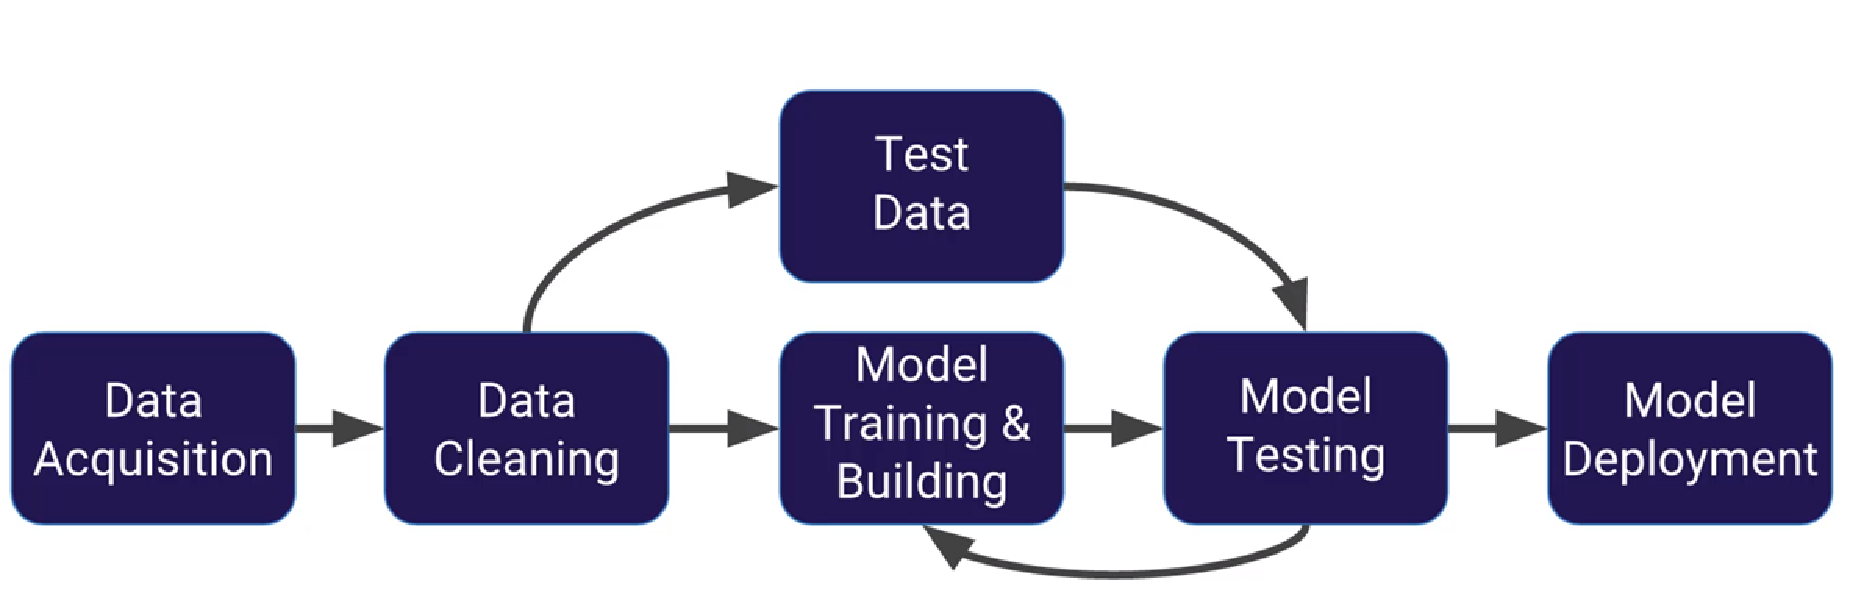
\includegraphics[scale=0.45]{./img/ml_process.pdf}
    \caption{Añadir img comparativa del Backtest vs Robotrader}
    \label{fig_mlp_13}
\end{figure}

Además de mostrar los datos teóricos que se hubiesen conseguido también he querido comparar con los datos de la simulación de Monte Carlo.

\begin{figure}[h]
    \centering
    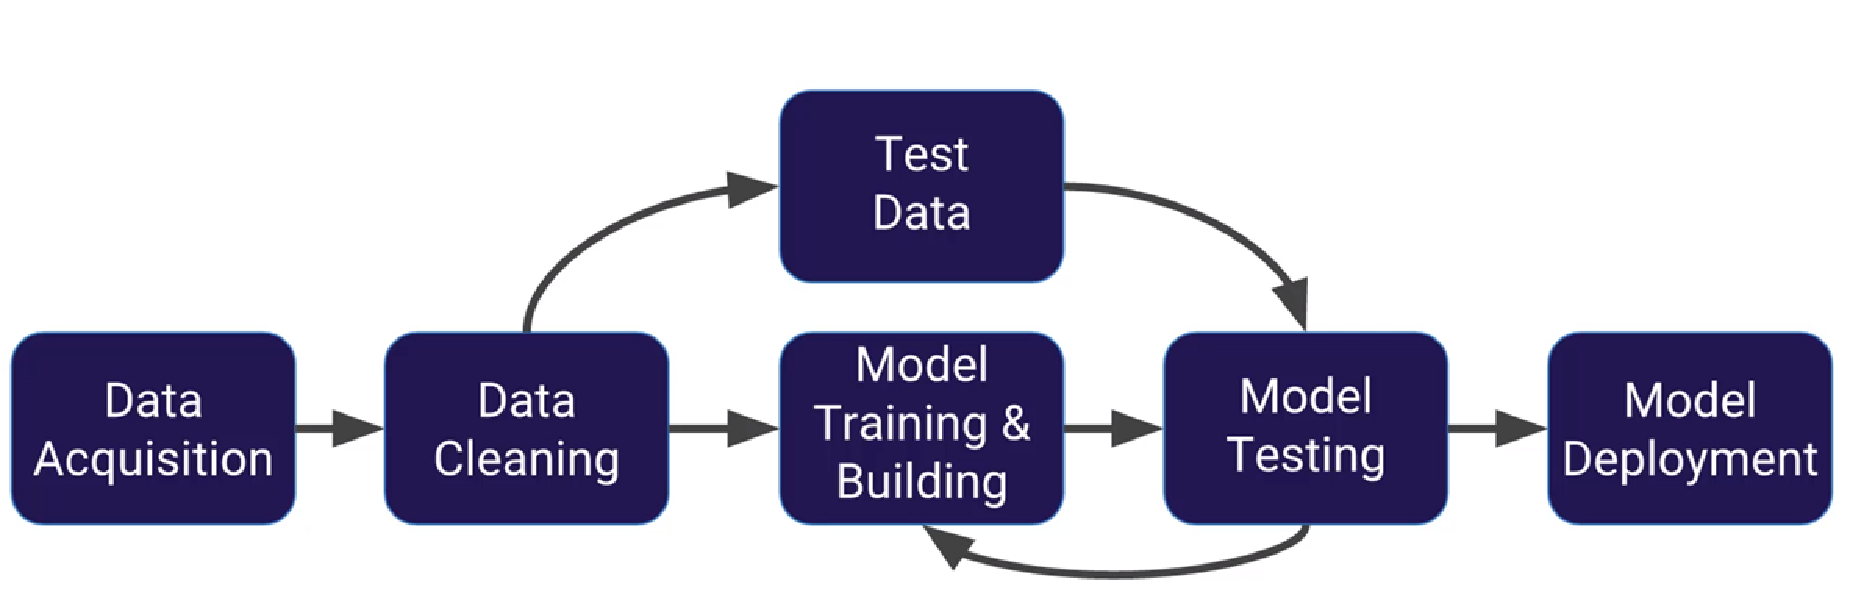
\includegraphics[scale=0.45]{./img/ml_process.pdf}
    \caption{Añadir img comparativa del Monte Carlo vs Robotrader}
    \label{fig_mlp_14}
\end{figure}

\begin{figure}[H]
    \centering
    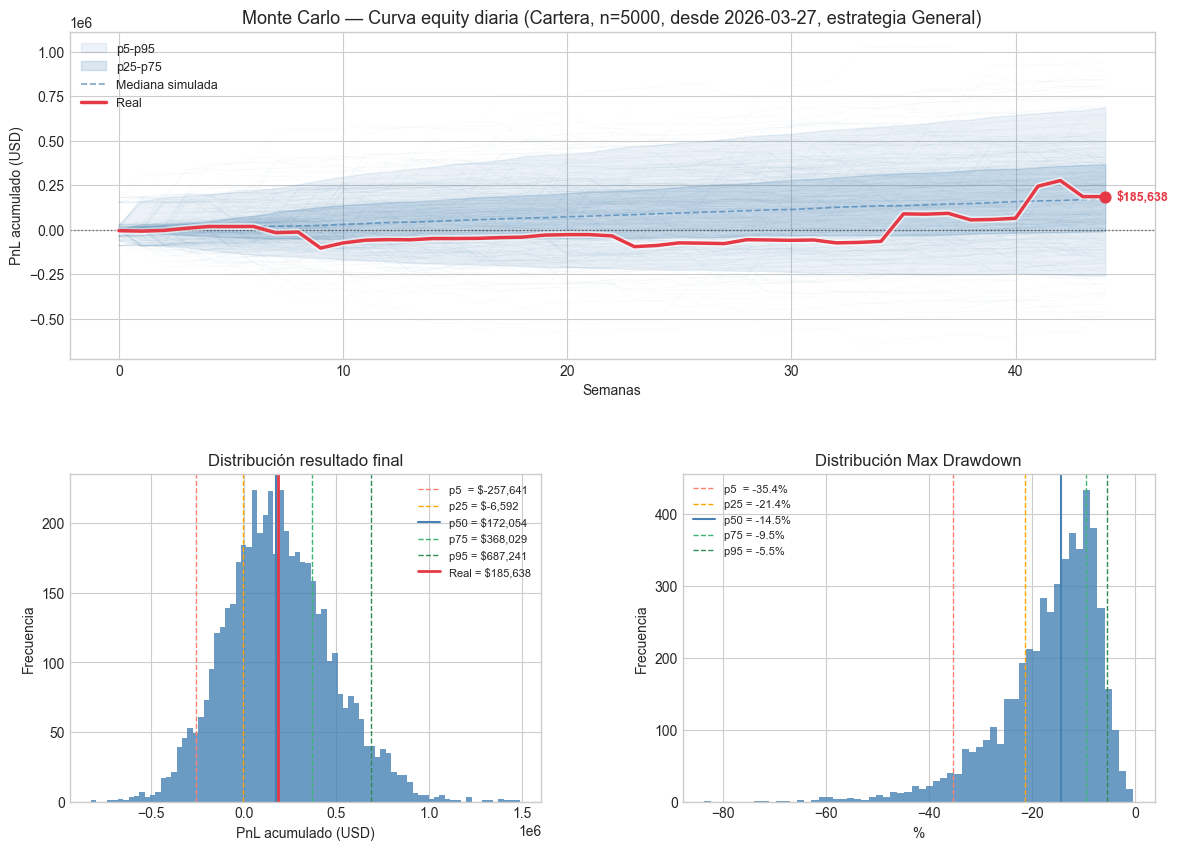
\includegraphics[width=\textwidth]{./img/monte_carlo_mal.png}
    \caption{Añadir img comparativa del Monte Carlo vs Robotrader}
    \label{fig_mlp_24}
\end{figure}

\begin{figure}[H]
    \centering
    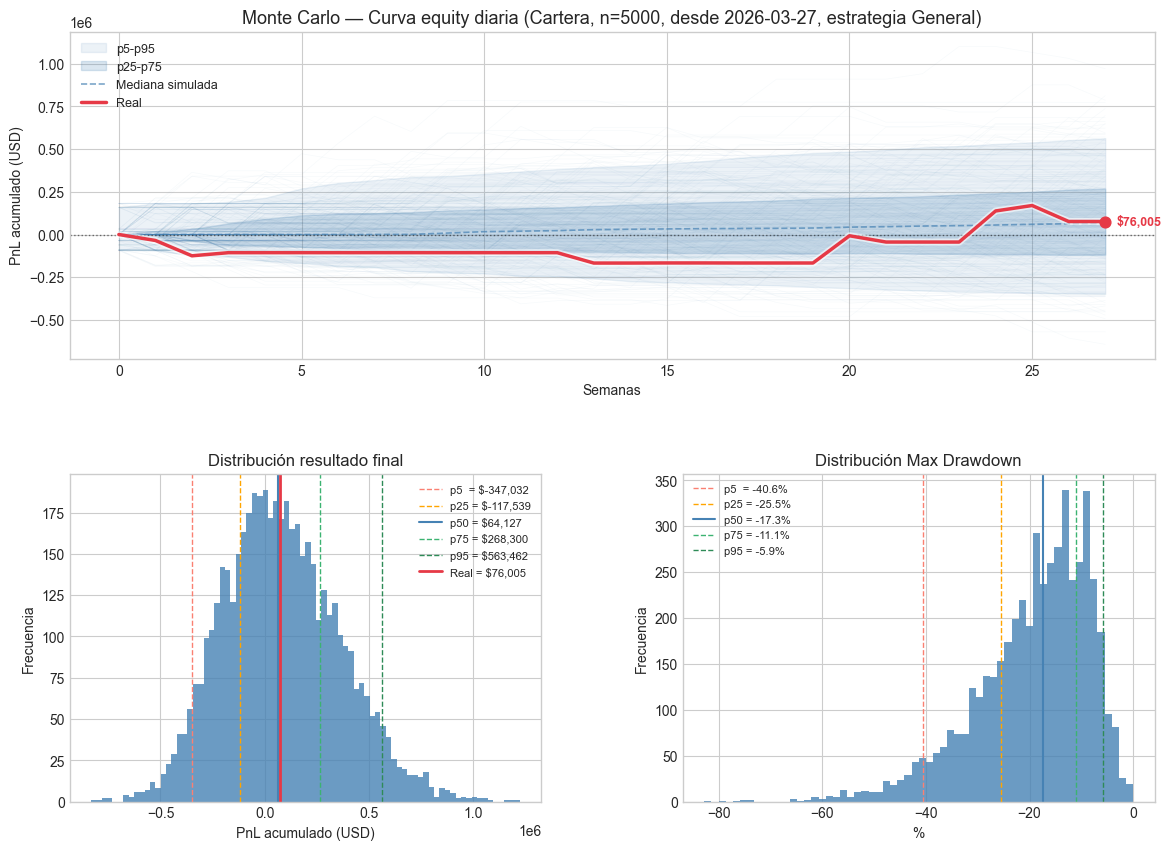
\includegraphics[width=\textwidth]{./img/monte_carlo_bien.png}
    \caption{Añadir img comparativa del Monte Carlo vs Robotrader}
    \label{fig_mlp_25}
\end{figure}

\notes{Añadir grafica de la evolución del equity, comparativa contra Robotrader} 

\notes{Añadir Monte Carlo}

\begin{table}[H]
\centering
\makebox[0pt]{%
\begin{tabular}{|c|c|c|c|c|c|c|}
\hline
\multirow{2}{*}{\textbf{Futuro}} &
\multirow{2}{*}{\textbf{Capital inicial}} &
\multicolumn{4}{c|}{\textbf{Capital final}} &
\multirow{2}{*}{\textbf{Ganancias mejor caso}} \\ \cline{3-6}
 & & \textbf{Normal} & \textbf{Scale-in} & \textbf{Sizing} & \textbf{Scale-in + Sizing} & \\ \hline

AD   & 30k  & \multicolumn{4}{c|}{No hay operaciones}                                                        & 0 \\ \hline
BP   & 30k  & \multicolumn{4}{c|}{Por alguna razón faltan dos features}                                      & 0 \\ \hline
CL   & 300k & \multicolumn{1}{c|}{305k}  & \multicolumn{1}{c|}{317k}   & \multicolumn{1}{c|}{306k}  & 400k   & \poscolor{100k} \\ \hline
EC   & 40k  & \multicolumn{4}{c|}{No hay operaciones}                                                        & 0 \\ \hline
ES   & 350k & \multicolumn{1}{c|}{320k}  & \multicolumn{1}{c|}{280k}   & \multicolumn{1}{c|}{349k}  & 250k   & \negcolor{-1k} \\ \hline
GC   & 450k & \multicolumn{1}{c|}{450k}  & \multicolumn{1}{c|}{465k}   & \multicolumn{1}{c|}{450k}  & 465k   & \poscolor{15k} \\ \hline
MFXI & 5k   & \multicolumn{1}{c|}{4.8k}  & \multicolumn{1}{c|}{4.75k}  & \multicolumn{1}{c|}{4.5k}  & 3.75k  & \negcolor{-0.2k} \\ \hline
NG   & 70k  & \multicolumn{1}{c|}{70k}   & \multicolumn{1}{c|}{69k}    & \multicolumn{1}{c|}{71k}   & 67k    & \poscolor{1k} \\ \hline
NQ   & 650k & \multicolumn{1}{c|}{630k}  & \multicolumn{1}{c|}{570k}   & \multicolumn{1}{c|}{650k}  & 550k   & 0 \\ \hline
YM   & 200k & \multicolumn{1}{c|}{198k}  & \multicolumn{1}{c|}{198k}   & \multicolumn{1}{c|}{200k}  & 196k   & 0 \\ \hline
ZB   & 50k  & \multicolumn{1}{c|}{50k}   & \multicolumn{1}{c|}{49k}    & \multicolumn{1}{c|}{50k}   & 48k    & 0 \\ \hline
ZN   & 30k  & \multicolumn{1}{c|}{25k}   & \multicolumn{1}{c|}{24k}    & \multicolumn{1}{c|}{22k}   & 0k     & \negcolor{-5k} \\ \hline
ZS   & 50k  & \multicolumn{1}{c|}{300k}  & \multicolumn{1}{c|}{300k}   & \multicolumn{1}{c|}{80k}   & 300k   & \poscolor{250k} \\ \hline

\end{tabular}

}
\caption{Tabla resumen de los 13 futuros evaluados en las cuatro modalidades operativas. Desde 2026-01-20 hasta 2026-06-01}
\end{table}

Como capital inicial he usado 10 veces el margin inicial mínimo para abrir una posición

% \begin{table}[H]
% \centering
% \makebox[0pt]{%
% \begin{tabular}{|c|c|c|c|c|c|c|}
% \hline
% \multirow{2}{*}{\textbf{Futuro}} &
% \multirow{2}{*}{\textbf{Capital inicial}} &
% \multicolumn{4}{c|}{\textbf{Capital final}} &
% \multirow{2}{*}{\textbf{Ganancias mejor caso}} \\ \cline{3-6}
%  & & \textbf{Normal} & \textbf{Scale-in} & \textbf{Sizing} & \textbf{Scale-in + Sizing} & \\ \hline

% CL   & 300k & \multicolumn{1}{c|}{300k}  & \multicolumn{1}{c|}{300k}   & \multicolumn{1}{c|}{300k}  & 300k   & 0 \\ \hline
% ES   & 350k & \multicolumn{1}{c|}{342k}  & \multicolumn{1}{c|}{345k}   & \multicolumn{1}{c|}{349k}  & 350k   & \negcolor{-1k} \\ \hline
% GC   & 450k & \multicolumn{1}{c|}{458k}  & \multicolumn{1}{c|}{452k}   & \multicolumn{1}{c|}{450k}  & 452k   & \poscolor{8k} \\ \hline
% MFXI & 5k   & \multicolumn{1}{c|}{4.8k}  & \multicolumn{1}{c|}{4.75k}  & \multicolumn{1}{c|}{4.5k}  & 3.75k  & \negcolor{-0.2k} \\ \hline
% NG   & 70k  & \multicolumn{1}{c|}{70k}   & \multicolumn{1}{c|}{69k}    & \multicolumn{1}{c|}{71k}   & 67k    & \poscolor{1k} \\ \hline
% NQ   & 650k & \multicolumn{1}{c|}{667.5k}& \multicolumn{1}{c|}{655k}   & \multicolumn{1}{c|}{650k}  & 655k   & \poscolor{17.5k} \\ \hline
% YM   & 200k & \multicolumn{1}{c|}{205k}  & \multicolumn{1}{c|}{205k}   & \multicolumn{1}{c|}{200k}  & 205k   & \poscolor{5k} \\ \hline
% ZB   & 50k  & \multicolumn{1}{c|}{50k}   & \multicolumn{1}{c|}{49k}    & \multicolumn{1}{c|}{49k}   & 49k    & 0 \\ \hline
% ZN   & 30k  & \multicolumn{1}{c|}{27.5k} & \multicolumn{1}{c|}{25k}    & \multicolumn{1}{c|}{24k}   & 0k     & \negcolor{-2.5k} \\ \hline
% ZS   & 50k  & \multicolumn{1}{c|}{-20k}  & \multicolumn{1}{c|}{-80k}   & \multicolumn{1}{c|}{48k}   & -80k   & \negcolor{-2k} \\ \hline

% \end{tabular}

% }
% \caption{Tabla resumen de los 13 futuros evaluados en las cuatro modalidades operativas. Desde 2026-03-27 hasta 2026-06-01, aunque Robotrader empezó el 6 para tener datos para las primeras predicciones}
% \end{table}

\begin{table}[H]
\centering
\makebox[0pt]{%
\begin{tabular}{|c|c|c|c|c|}
\hline
\textbf{Futuro} & \textbf{Capital inicial} & \textbf{Ganancias mejor caso} & \textbf{Max DD} & \textbf{Ratio} \\ \hline
CL   & 300k & 0                        &  &  \\ \hline
ES   & 350k & \negcolor{-1k}           &  &  \\ \hline
GC   & 450k & \poscolor{8510}            & 6730 & 1.26 \\ \hline
MFXI & 5k   & \negcolor{-0.2k}         &  &  \\ \hline
NG   & 70k  & \poscolor{904}            & 2116.23 & 0.43 \\ \hline
NQ   & 650k & \poscolor{17385}         & 0 & No aplica \\ \hline
YM   & 200k & \poscolor{6825}            & 2375.0 & 2.87 \\ \hline
ZB   & 50k  & 0                        &  &  \\ \hline
ZN   & 30k  & \negcolor{-2.5k}         &  &  \\ \hline
ZS   & 50k  & \negcolor{-2k}           &  &  \\ \hline
\end{tabular}


}
\caption{Tabla resumen de los 13 futuros evaluados en las cuatro modalidades operativas. Desde 2026-03-27 hasta 2026-06-01, aunque Robotrader empezó el 6 para tener datos para las primeras predicciones}
\end{table}

En ganancias absolutas séptimo/noveno en la competición de 58 personas.

\subsection{Análisis de resultados de entrenamiento}

\begin{figure}[H]
\centering

\begin{minipage}{0.48\textwidth}
    \centering
    
\includegraphics[width=\linewidth]{../../TradingBots/Models/ad/classification_report_LSTM.png}
    
    (a) Classification report
\end{minipage}
\hfill
\begin{minipage}{0.48\textwidth}
    \centering
    
\includegraphics[width=\linewidth]{../../TradingBots/Models/ad/auc_roc_reliability_LSTM.png}
    
    (b) ROC y reliability curve
\end{minipage}

\vspace{0.3cm}

\begin{minipage}{0.48\textwidth}
    \centering
    
\includegraphics[width=\linewidth]{../../TradingBots/Models/ad/regression_LSTM.png}
    
    (c) MAE y regresión
\end{minipage}
\hfill
\begin{minipage}{0.48\textwidth}
    \centering
    
\includegraphics[width=\linewidth]{../../TradingBots/Models/ad/loss_LSTM.png}
    
    (d) Loss
\end{minipage}

\caption{Resultados obtenidos por el modelo LSTM.}
\label{fig:lstm_results}

\end{figure}

\begin{figure}[H]
\centering

\begin{minipage}{0.48\textwidth}
    \centering
    
\includegraphics[width=\linewidth]{../../TradingBots/Models/ad/classification_report_GRU.png}
    
    (a) Classification report
\end{minipage}
\hfill
\begin{minipage}{0.48\textwidth}
    \centering
    
\includegraphics[width=\linewidth]{../../TradingBots/Models/ad/auc_roc_reliability_GRU.png}
    
    (b) ROC y reliability curve
\end{minipage}

\vspace{0.3cm}

\begin{minipage}{0.48\textwidth}
    \centering
    
\includegraphics[width=\linewidth]{../../TradingBots/Models/ad/regression_GRU.png}
    
    (c) MAE y regresión
\end{minipage}
\hfill
\begin{minipage}{0.48\textwidth}
    \centering
    
\includegraphics[width=\linewidth]{../../TradingBots/Models/ad/loss_GRU.png}
    
    (d) Loss
\end{minipage}

\caption{Resultados obtenidos por el modelo GRU.}
\label{fig:gru_results}

\end{figure}

\todo{Añadir curva auc roc para las dos capas de clasificación}

\todo{Añadir curva loss por fold}

\begin{figure}[H]
    \centering
    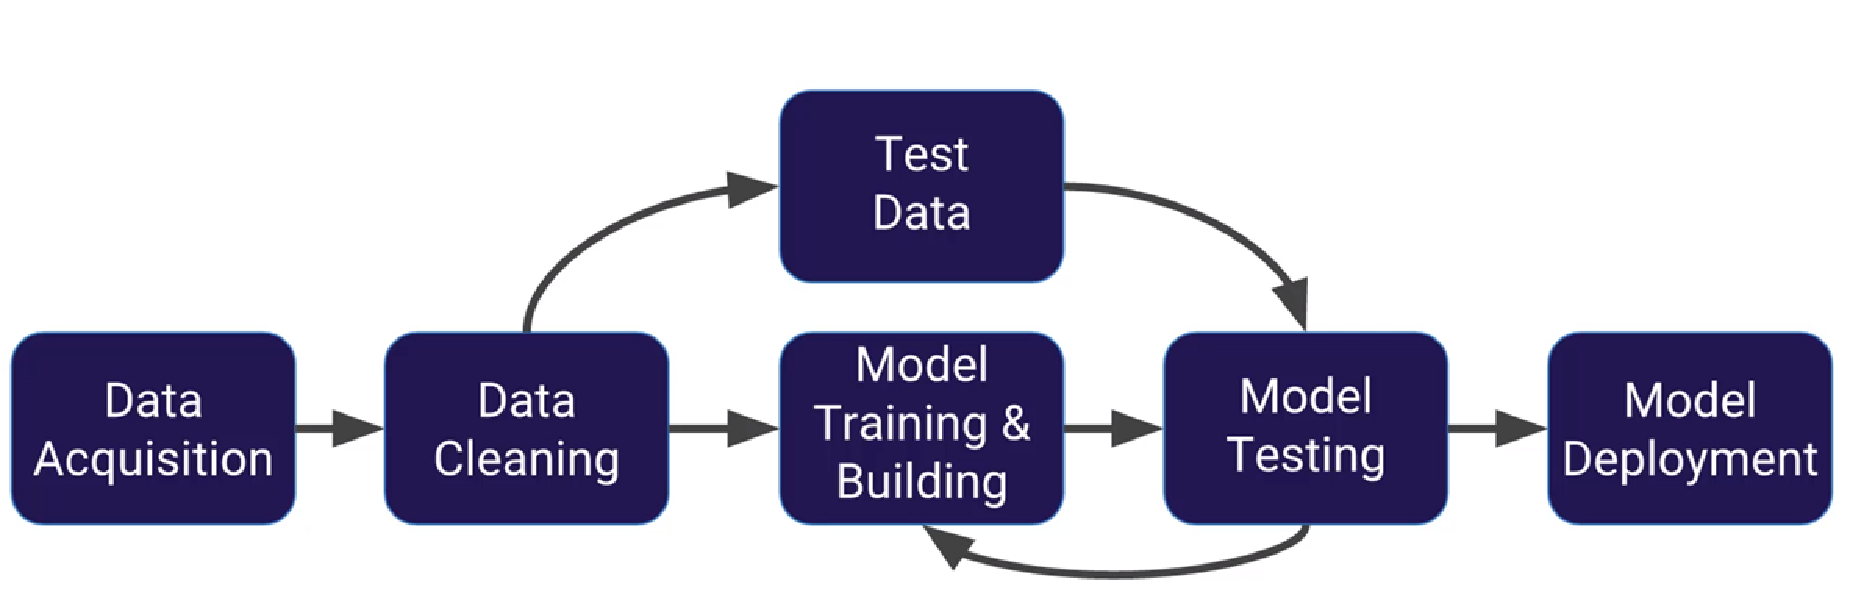
\includegraphics[scale=0.45]{./img/ml_process.pdf}
    \caption{Añadir img con evolución de las métricas dependiendo de los umbrales}
    \label{fig_mlp_18}
\end{figure}

% \begin{figure}[H]
%     \centering
%     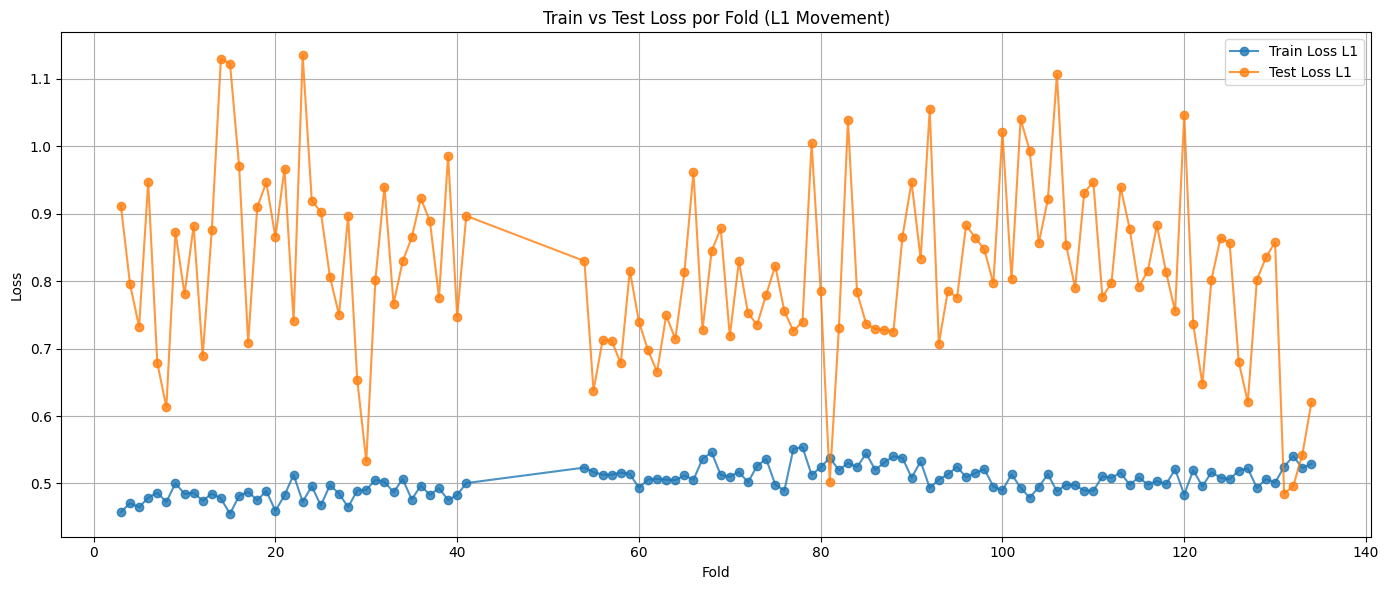
\includegraphics[width=\textwidth]{./img/loss.png}
%     \caption{Evolución de la función de pérdida en la última época de cada fold}
%     \label{fig_mlp_21}
% \end{figure}

\begin{figure}[h]
    \centering
    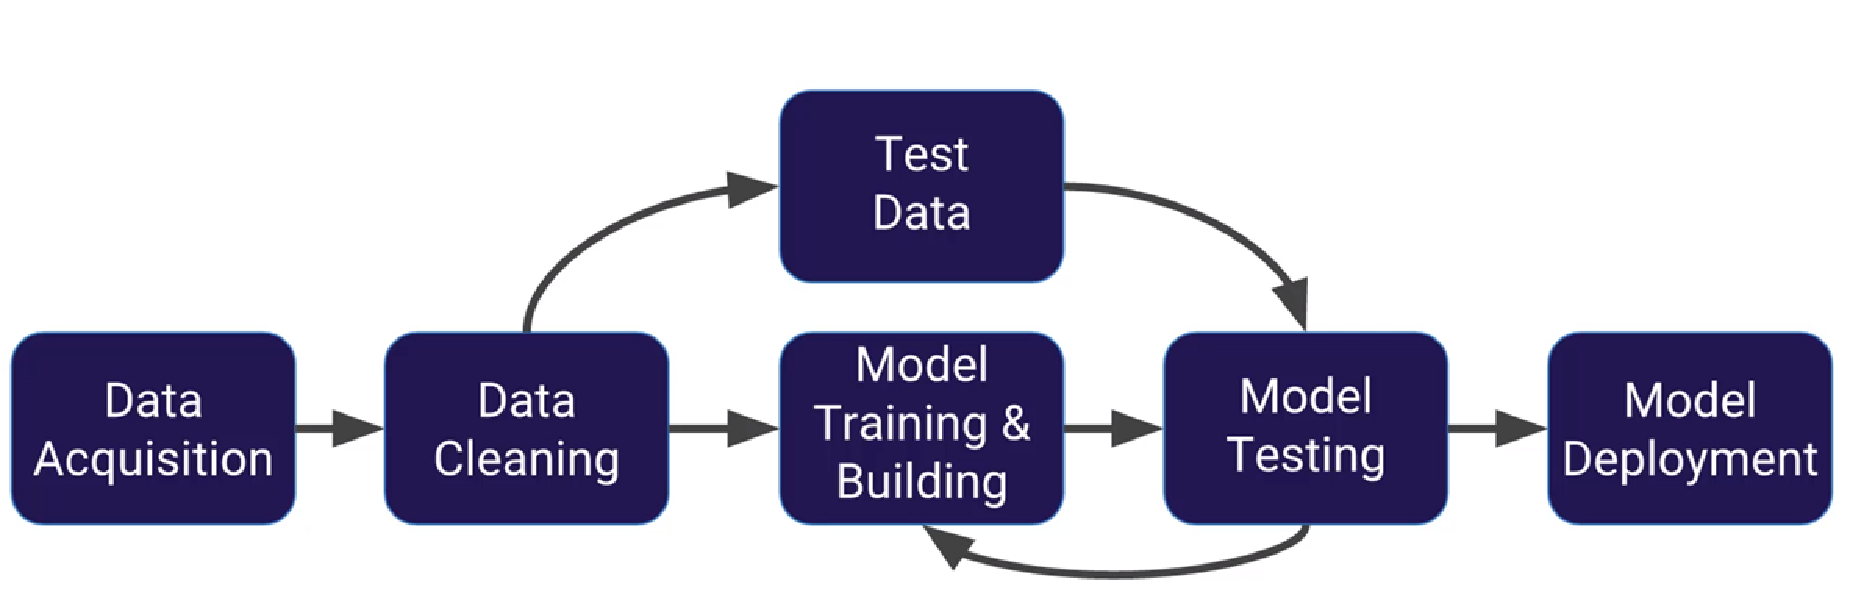
\includegraphics[scale=0.45]{./img/ml_process.pdf}
    \caption{Añadir img con una simulación de Monte Carlo con los percentiles}
    \label{fig_mlp_19}
\end{figure}

\subsection{Análisis de resultados de optimización, Backtest de la cartera y Simulación de Monte Carlo}

Una vez obtenidas las señales optimizadas para cada futuro, se realiza un análisis conjunto del comportamiento de la cartera completa. El objetivo es evaluar si la combinación de activos mejora el rendimiento respecto a operar únicamente un activo individual, así como estudiar la robustez del sistema bajo diferentes secuencias de resultados.

Para ello se lleva a cabo un nuevo backtest a nivel de cartera. En este proceso se cargan todos los \textit{trades} generados por cada futuro utilizando la estrategia operativa óptima obtenida previamente. A continuación, se construye un único \textit{DataFrame} que agrupa todas las operaciones por fecha, lo que permite simular la evolución conjunta del capital.

La simulación se realiza sobre una cuenta con un capital inicial de 1\,000\,000 USD, lo que permite incorporar restricciones realistas de riesgo y liquidez. En particular, se tienen en cuenta:

\begin{itemize}
    \item los márgenes iniciales y de mantenimiento de cada futuro,
    \item el valor nocional de cada contrato,
    \item el porcentaje máximo de capital que puede arriesgarse por operación,
    \item la exposición total máxima permitida, fijada en un 25\% del capital inicial.
\end{itemize}

Las predicciones se ordenan por nivel de confianza total y se procesan secuencialmente, verificando en cada caso que la operación no exceda los límites de margen ni las restricciones de exposición. Solo las operaciones que cumplen estas condiciones se ejecutan en la simulación.

Además del backtest, se realiza una simulación de Monte Carlo adicional para evaluar la dispersión de las métricas de la cartera completa. Para ello se agrupan los PnL diarios de todos los activos y se aplica un \textit{overlapping block bootstrap}, remuestreando bloques solapados de la serie diaria de beneficios. Este enfoque permite preservar parte de la estructura temporal y generar múltiples trayectorias alternativas del rendimiento de la cartera.

El análisis conjunto del backtest y de la simulación de Monte Carlo permite comparar el rendimiento de la cartera diversificada frente a la operativa de un único activo, así como evaluar la estabilidad del sistema bajo diferentes escenarios de mercado.


\setlength{\parindent}{0em}

\chapter{Conclusiones y líneas futuras}\label{cap5}\thispagestyle{fancy}

\vspace{-1.3cm}

\section{Conclusiones}

\section{Líneas futuras}

Por limitaciones del tiempo dejo pendiente dos mejoras

Por una parte añadir una interfaz gráfica independiente de grafana para tener personalización total

Y por otra parte añadir en esa misma página un chatbot usando RASA o un LLM para responder preguntas a partir de toda la información disponible

\setlength{\parindent}{0em}

\chapter{Aspectos éticos, económicos, sociales y ambientales}\label{cap6}\thispagestyle{fancy}

\vspace{-1.3cm}

\section{Introducción}

Desde el punto de vista económico el sistema tiene influencia en la reducción de costes necesarios para operar una cartera de activos, permitiendo a
profesionales autónomos o quienes lo toman como un hobby. En el ámbito ético y social, . Y por último, con respecto al impacto ambiental, este sistema
no tiene casi impacto al poder ejecutarse en local en hardware particular no profesional.

\section{Descripción de impactos relevantes relacionados con el proyecto}

\begin{description}
    \item[Impacto económico]  \hfill \\
        1
    \item[Impacto ético y social]  \hfill \\
        2
    \item[Impacto ambiental]  \hfill \\
        3
\end{description}

\section{Análisis detallado de alguno de los principales impactos}

El impacto mayoritario de este proyecto se centra en el tema económico

\section{Conclusiones}

Como conclusión final

\setlength{\parindent}{0em}

\chapter{Presupuesto económico}\label{cap7}\thispagestyle{fancy}

\vspace{-1.3cm}

%En la normativa del TFG del GISD se establece que la memoria del TFG debe incluir un presupuesto económico”. A modo de ejemplo, la tabla del presupuesto de un proyecto podría ser la siguiente:

% \begin{table}[ht]
% \centering
% \rotatebox{90}{
% \resizebox{0.76\textheight}{!}{
% \begin{tabular}{|p{1.5cm}|p{1.5cm}|p{1.5cm}|p{1.5cm}|p{1.5cm}|p{1.5cm}|p{1.5cm}|p{1.5cm}|p{1.5cm}}
% \hline
% \multicolumn{5}{|l|}{\textbf{COSTE DE MANO DE OBRA (coste directo)}} & \multicolumn{2}{c|}{\textbf{Horas}} & \multicolumn{1}{c|}{\textbf{Precio/hora}} & \multicolumn{1}{c|}{\textbf{Total}} \\ \hline
% \multicolumn{5}{c}{} & \multicolumn{2}{|c|}{360} & \multicolumn{1}{c|}{15 €} & \multicolumn{1}{c|}{\textbf{5.400 €}} \\ \cline{6-9}
% \multicolumn{4}{l}{} &  & \multicolumn{2}{l}{} &  &  \\ \hline
% \multicolumn{4}{|l|}{\textbf{COSTE DE RECURSOS MATERIALES (coste directo)}} & \multicolumn{1}{c|}{\textbf{\begin{tabular}[c]{@{}c@{}}Precio \\ de compra\end{tabular}}} & \multicolumn{2}{c|}{\textbf{\begin{tabular}[c]{@{}c@{}}Uso en \\ meses\end{tabular}}} & \multicolumn{1}{c|}{\textbf{\begin{tabular}[c]{@{}c@{}}Amortización \\ (en años)\end{tabular}}} & \multicolumn{1}{c|}{\textbf{Total}} \\ \hline
% \multicolumn{4}{|l|}{Ordenador personal (Software incluido)} & \multicolumn{1}{c|}{1.500,00 €} & \multicolumn{2}{c|}{6} & \multicolumn{1}{c|}{5} & \multicolumn{1}{c|}{\textbf{150,00 €}} \\ \hline
% \multicolumn{4}{|l|}{Impresora láser} & \multicolumn{1}{c|}{500,00 €} & \multicolumn{2}{c|}{6} & \multicolumn{1}{c|}{5} & \multicolumn{1}{c|}{\textbf{50,00 €}} \\ \hline
% \multicolumn{4}{|l|}{Otro equipamiento} & \multicolumn{1}{c|}{} & \multicolumn{2}{c|}{X} & \multicolumn{1}{c|}{X} & \multicolumn{1}{c|}{X €} \\ \hline
% \multicolumn{4}{l}{} &  & \multicolumn{2}{l}{} &  &  \\ \hline
% \multicolumn{8}{|l|}{\textbf{COSTE TOTAL DE RECURSOS MATERIALES}} & \multicolumn{1}{c|}{\textbf{200,00 €}} \\ \hline
% \multicolumn{2}{l}{} & \multicolumn{2}{l}{} & \multicolumn{2}{l}{} & \multicolumn{2}{l}{} &  \\ \hline
% \multicolumn{2}{|l|}{\textbf{GASTOS GENERALES (costes indirectos)}} & \multicolumn{2}{c|}{15\%} & \multicolumn{4}{c|}{sobre CD} & \multicolumn{1}{c|}{\textbf{840,00 €}} \\ \hline
% \multicolumn{2}{|l|}{\textbf{BENEFICIO INDUSTRIAL}} & \multicolumn{2}{c|}{6\%} & \multicolumn{4}{c|}{sobre CD+CI} & \multicolumn{1}{c|}{\textbf{336.00 €}} \\ \hline
% \multicolumn{2}{l}{} & \multicolumn{2}{l}{} & \multicolumn{2}{l}{} & \multicolumn{2}{l}{} &  \\ \hline
% \multicolumn{9}{|l|}{\textbf{MATERIAL FUNGIBLE}} \\ \hline
% \multicolumn{8}{|l|}{Impresión} & \multicolumn{1}{c|}{\textbf{100,00 €}} \\ \hline
% \multicolumn{8}{|l|}{Encuadernación} & \multicolumn{1}{c|}{\textbf{300,00 €}} \\ \hline
% \multicolumn{2}{l}{} & \multicolumn{2}{l}{} & \multicolumn{2}{l}{} & \multicolumn{2}{l}{} &  \\ \hline
% \multicolumn{8}{|l|}{\textbf{SUBTOTAL PRESUPUESTO}} & \multicolumn{1}{c|}{\textbf{7.176,00 €}} \\ \hline
% \multicolumn{7}{|l|}{\textbf{IVA APLICABLE}} & \multicolumn{1}{c|}{21\%} & \multicolumn{1}{c|}{\textbf{1.507,00 €}} \\ \hline
% \multicolumn{8}{|l|}{\textbf{TOTAL PRESUPUESTO}} & \multicolumn{1}{c|}{\textbf{8.683,00 €}} \\ \hline
% \end{tabular}}}
% \label{tab:presupuesto}
% \end{table}
\afterpage{
\clearpage
\thispagestyle{empty}
\begin{landscape}

\begin{table}[ht]
\centering
\resizebox{\linewidth}{!}{
\begin{tabular}{|p{1.5cm}|p{1.5cm}|p{1.5cm}|p{1.5cm}|p{1.5cm}|p{1.5cm}|p{1.5cm}|p{1.5cm}|p{1.5cm}}
\hline
\multicolumn{5}{|l|}{\textbf{COSTE DE MANO DE OBRA (coste directo)}} & \multicolumn{2}{c|}{\textbf{Horas}} & \multicolumn{1}{c|}{\textbf{Precio/hora}} & \multicolumn{1}{c|}{\textbf{Total}} \\ \hline
\multicolumn{5}{c}{} & \multicolumn{2}{|c|}{360} & \multicolumn{1}{c|}{15 €} & \multicolumn{1}{c|}{\textbf{5.400 €}} \\ \cline{6-9}
\multicolumn{4}{l}{} &  & \multicolumn{2}{l}{} &  &  \\ \hline
\multicolumn{4}{|l|}{\textbf{COSTE DE RECURSOS MATERIALES (coste directo)}} & \multicolumn{1}{c|}{\textbf{\begin{tabular}[c]{@{}c@{}}Precio \\ de compra\end{tabular}}} & \multicolumn{2}{c|}{\textbf{\begin{tabular}[c]{@{}c@{}}Uso en \\ meses\end{tabular}}} & \multicolumn{1}{c|}{\textbf{\begin{tabular}[c]{@{}c@{}}Amortización \\ (en años)\end{tabular}}} & \multicolumn{1}{c|}{\textbf{Total}} \\ \hline
\multicolumn{4}{|l|}{Ordenador personal (Software incluido)} & \multicolumn{1}{c|}{1.500,00 €} & \multicolumn{2}{c|}{6} & \multicolumn{1}{c|}{5} & \multicolumn{1}{c|}{\textbf{150,00 €}} \\ \hline
\multicolumn{4}{|l|}{Impresora láser} & \multicolumn{1}{c|}{500,00 €} & \multicolumn{2}{c|}{6} & \multicolumn{1}{c|}{5} & \multicolumn{1}{c|}{\textbf{50,00 €}} \\ \hline
\multicolumn{4}{|l|}{Otro equipamiento} & \multicolumn{1}{c|}{} & \multicolumn{2}{c|}{X} & \multicolumn{1}{c|}{X} & \multicolumn{1}{c|}{X €} \\ \hline
\multicolumn{4}{l}{} &  & \multicolumn{2}{l}{} &  &  \\ \hline
\multicolumn{8}{|l|}{\textbf{COSTE TOTAL DE RECURSOS MATERIALES}} & \multicolumn{1}{c|}{\textbf{200,00 €}} \\ \hline
\multicolumn{2}{l}{} & \multicolumn{2}{l}{} & \multicolumn{2}{l}{} & \multicolumn{2}{l}{} &  \\ \hline
\multicolumn{2}{|l|}{\textbf{GASTOS GENERALES (costes indirectos)}} & \multicolumn{2}{c|}{15\%} & \multicolumn{4}{c|}{sobre CD} & \multicolumn{1}{c|}{\textbf{840,00 €}} \\ \hline
\multicolumn{2}{|l|}{\textbf{BENEFICIO INDUSTRIAL}} & \multicolumn{2}{c|}{6\%} & \multicolumn{4}{c|}{sobre CD+CI} & \multicolumn{1}{c|}{\textbf{336.00 €}} \\ \hline
\multicolumn{2}{l}{} & \multicolumn{2}{l}{} & \multicolumn{2}{l}{} & \multicolumn{2}{l}{} &  \\ \hline
\multicolumn{9}{|l|}{\textbf{MATERIAL FUNGIBLE}} \\ \hline
\multicolumn{8}{|l|}{Impresión} & \multicolumn{1}{c|}{\textbf{100,00 €}} \\ \hline
\multicolumn{8}{|l|}{Encuadernación} & \multicolumn{1}{c|}{\textbf{300,00 €}} \\ \hline
\multicolumn{2}{l}{} & \multicolumn{2}{l}{} & \multicolumn{2}{l}{} & \multicolumn{2}{l}{} &  \\ \hline
\multicolumn{8}{|l|}{\textbf{SUBTOTAL PRESUPUESTO}} & \multicolumn{1}{c|}{\textbf{7.176,00 €}} \\ \hline
\multicolumn{7}{|l|}{\textbf{IVA APLICABLE}} & \multicolumn{1}{c|}{21\%} & \multicolumn{1}{c|}{\textbf{1.507,00 €}} \\ \hline
\multicolumn{8}{|l|}{\textbf{TOTAL PRESUPUESTO}} & \multicolumn{1}{c|}{\textbf{8.683,00 €}} \\ \hline
\end{tabular}}
\label{tab:presupuesto}
\end{table}
\end{landscape}
\clearpage
}

%%%%% ESTILO DEL DOCUMENTO %%%%%%%


%%%%%%%%%%%%%%%%%%%%%%%%%%%%%%%%%%%%%%

%% Bibliografía. Usa el ref.bib 
\clearpage

%\nocite{*}

\Urlmuskip=0mu plus 1mu\relax

\addcontentsline{toc}{chapter}{Bibliografía}
\bibliography{ref.bib}
\bibliographystyle{ieeetr}

%% Anexos
\chapter*{Anexos}% If \appendix doesn't insert a \chapter
\addcontentsline{toc}{chapter}{Anexos}% Print Appendix in ToC
\setcounter{section}{0}% Reset numbering for sections
\renewcommand{\thesection}{\Alph{section}}% Adjust section printing (from here onward)

\setlength{\parindent}{0em}

\section{XXXXXXXXXXXXXXXX}\label{anexoA}


\clearpage

\end{document}
